%%%%%%%%%%%%%%% Start of Title Page %%%%%%%%%%%
\begin{titlepage}
    \begin{center}
        \textit{Heaven's Light is Our Guide}
        \\[0.5cm]
        \textbf{\Large Rajshahi University of Engineering \& Technology}
        \\[0.3cm]
        \textbf{\large Department of Electronics \& Telecommunication Engineering}
        \\[0.2cm]
        \begin{figure}[!htbp]
            \centering
            
\includegraphics[scale=0.3]{src/logo_ruet}
            \label{fig:RUET logo}
        \end{figure}
        \textbf{\Large ETE 1212: Sessional Based on ETE 1211 }
        \\[0.5cm]
        \myrule[1pt][5pt]

        %%%%%%%%%%%%%%%%%%%%%%%%%%%%%%%%%%%%%%%%%%%%%%%
        %%%%%%%%%%%%%%% STUDENT'S INFO %%%%%%%%%%%%%%%%
        %%%%%%%%%%%%%%%%%%%%%%%%%%%%%%%%%%%%%%%%%%%%%%%

        \textbf{\Large  Experiment No. 02}
        \\[.25cm]
        \textbf{\large Experimental study on V-I characteristics curve of a diode and implementation of diode series parallel circuit with LED}
        \\
        \myrule[1pt][5pt]
        \begin{minipage}{0.4\textwidth}
            \vspace{0.5cm}
            \begin{flushleft}
                \emph{\textbf{\large Submitted by:}}
                \\
                Shahoriar Rahman \\
                Roll: 2104001 \\
                Session: 2021-22
            \end{flushleft}
        \end{minipage}
        ~
        \begin{minipage}{0.4\textwidth}
            \vspace{0.5cm}
            \begin{flushright}
                \emph{\textbf{\large Submitted to:}}
                \\
                Hasan Sarker
                \\
                Lecturer
                \\
                Dept. of ETE, RUET
                \\
            \end{flushright}
        \end{minipage}\\[0.7cm]
        \makeatother

        \textbf{Date of Experiment : 16/07/2023}\\
        \textbf{Date of Submission : 22/07/2023}\\[1cm]

        %************** End of Student's Info *********


        \vfill
        %%%%%%%%%%%%%%% TEACHER SECTION %%%%%%%%%%%%%%%
        \hrulefill
        \vspace{-5mm}
        \begin{multicols}{3}
            \begin{itemize} [labelindent=3em,labelsep=0.5cm,leftmargin=*,noitemsep]
                \item[] \textbf{\underline{Report}}
                \item[$\square$] Excellent
                \item[$\square$] Very Good
                \item[$\square$] Good
                \item[$\square$] Average
                \item[$\square$] Poor
            \end{itemize}
            \columnbreak
            \textbf{(Teacher's Section)}
            \\[1.5cm]
            --------------------------------
            \\
            Signature
            \columnbreak
            \begin{itemize}
                [labelindent=6em,labelsep=0.5cm,leftmargin=*,noitemsep]
                \item[] \textbf{\underline{Viva}}
                \item[$\square$] Excellent
                \item[$\square$] Very Good
                \item[$\square$] Good
                \item[$\square$] Average
                \item[$\square$] Poor
            \end{itemize}
        \end{multicols}
    \end{center}
\end{titlepage}

%************** End of Teacher Section ********
%************** End of Title Page *************


%%%%%%%%%%%%%%% Exp. Positioning %%%%%%%%%%%%%%
\titleformat{\chapter}[display]
{\normalfont\large\bfseries}{Experiment No: \thechapter}{0pt}{\large}

\titlespacing*{\chapter}{0pt}{-15pt}{10pt}
% \addcontentsline{lof}{chapter}{\protect\numberline{ \ref{exp1}}}
% \addcontentsline{lot}{chapter}{\protect\numberline{ \ref{exp1}}}
%************** End of Exp. Positioning *******


%%%%%%%%%%%%%%%%%%%%%%%%%%%%%%%%%%%%%%%%%%%%%%%
%%%%%%%%%%%%%%% Student's Part %%%%%%%%%%%%%%%%
%%%%%%%%%%%%%%% Start of Report %%%%%%%%%%%%%%%
%%%%%%%%%%%%%%%%%%%%%%%%%%%%%%%%%%%%%%%%%%%%%%%


%**********************************************
\chapter{Experiment Name: Experimental study on V-I characteristics curve of a diode and implementation of diode series parallel circuit with LED}
\label{exp1}


%**********************************************
\section{Objectives}
The main objectives of this experiment are
\begin{enumerate}
    \item To observe how the voltage and current works in a diode
    \item To know the fundamentals of diode
    \item To know how to plot graphs of various ratios
    \item To create circuits with LED on the projection board
\end{enumerate}

\section{Theory}
\subsection{Diode}
A diode is a semiconductor device with vital functionalities in electronics. Its working principle relies on the interaction between P-type and N-type semiconductor materials. When a voltage is applied across the diode in the forward bias, the P-side becomes positively charged, and the N-side becomes negatively charged, allowing current to flow freely. Conversely, in the reverse bias, the P-side becomes negatively charged, and the N-side becomes positively charged, blocking the current flow. This unidirectional behavior enables diodes to act as rectifiers, converting AC to DC, and as voltage regulators, protecting circuits from reverse voltage. Additionally, they play a crucial role in signal demodulation and light-emitting processes in LEDs.
\begin{figure}[H]
    \centering
    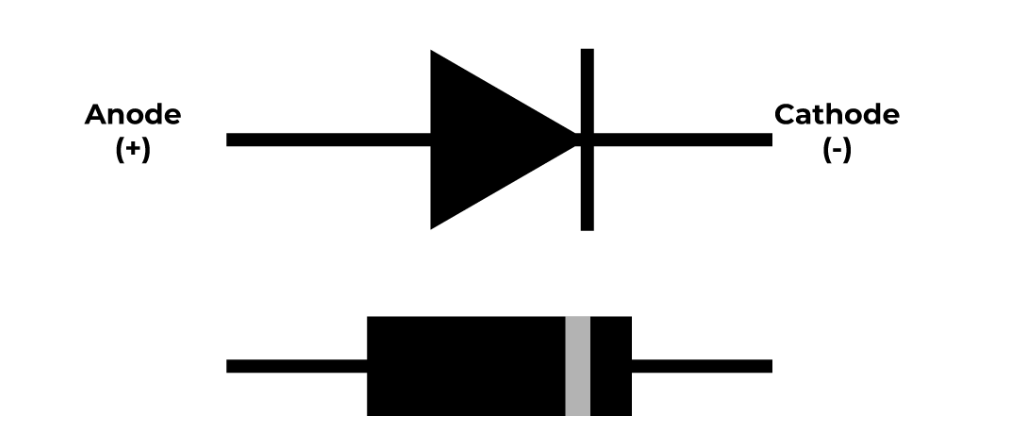
\includegraphics[scale=0.15]{src/exp02/diode.png}
    \caption{Diode symbol}
\end{figure}

\subsection{Forward Bias}
When the external voltage is applied across the P-N junction diode, this is known as forward
bias or biasing. The P-side of the diode is connected to the positive terminal, and the N-
side is fastened to the battery’s negative side in a forward bias setup. The junction barrier
potential is opposite to the applied voltage in this instance.
\begin{figure}[H]
    \centering
    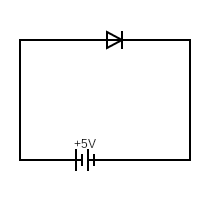
\includegraphics[scale=0.6]{src/exp02/circuit (3).png}
    \caption{Forward Bias of Diode}
\end{figure}
\subsection{Reverse Bias}
Reverse bias refers to the application of an external voltage across a semiconductor diode
such that the positive terminal of the battery is connected to the n-side and the negative
terminal is connected to the p-side of the diode.
\begin{figure}[H]
    \centering
    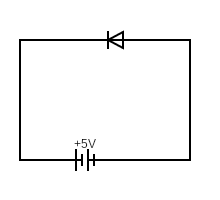
\includegraphics[scale=0.6]{src/exp02/circuit (4).png}
    \caption{Reverse Bias of Diode}
\end{figure}

\section{Required Components}
\begin{enumerate}
    \item P-N Junction Diode
    \item Resistors(3 pieces;1k ohm,100 ohm,100 ohm)
    \item Project Board
    \item LED (3 pieces))
    \item Signal Generator
    \item Multimeter
    \item Jumper Cables
\end{enumerate}

\section{Circuit Diagram}
\begin{figure}[H]
    \centering
    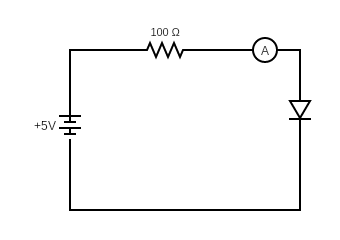
\includegraphics[scale=0.6]{src/exp02/circuit (5).png}
    \caption{Circuit Diagram with single 100 ohm resistor}
\end{figure}

\begin{figure}[H]
    \centering
    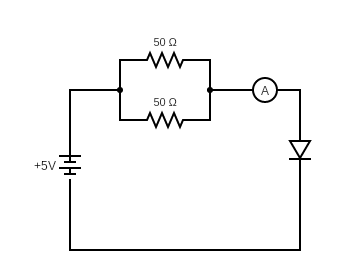
\includegraphics[scale=0.6]{src/exp02/circuit (7).png}
    \caption{Circuit Diagram with two 50 ohm resistors connected in parallel}
\end{figure}

\begin{figure}[H]
    \centering
    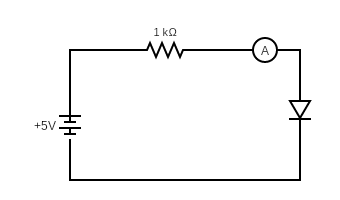
\includegraphics[scale=0.6]{src/exp02/circuit (8).png}
    \caption{Circuit Diagram with one single 1k $\Omega $ resistor}
\end{figure}

\section{Experimental Data}
\begin{figure}[htbp]
    \begin{minipage}{0.3\textwidth}
        \centering
        \begin{tabular}{|c|c|c|}
            \hline
            \textbf{\boldmath{SL}} & \textbf{\boldmath{$\text{V}_ \text{in}$}} & \textbf{\boldmath{$\text{I}_ \text{out}$}} \\ \hline
            1                      & 0                                         & 0                                          \\ \hline
            2                      & 1.04                                      & 0.001                                      \\ \hline
            3                      & 1.77                                      & 0.002                                      \\ \hline
            4                      & 2.33                                      & 0.003                                      \\ \hline
            5                      & 2.67                                      & 0.004                                      \\ \hline
            6                      & 3.38                                      & 0.005                                      \\ \hline
            7                      & 4.04                                      & 0.006                                      \\ \hline
            8.                     & 5.03                                      & 0.008                                      \\ \hline
            9                      & 5.82                                      & 0.009                                      \\ \hline
            10                     & 8.12                                      & 0.01                                       \\ \hline
        \end{tabular}
        \subcaption{Data for 50 ohm}
        \label{tab:table1}
    \end{minipage}%
    \hfill
    \begin{minipage}{0.3\textwidth}
        \centering
        \begin{tabular}{|c|c|c|}
            \hline
            \textbf{\boldmath{SL}} & \textbf{\boldmath{$\text{V}_ \text{in}$}} & \textbf{\boldmath{$\text{I}_ \text{out}$}} \\ \hline
            1                      & 0                                         & 0                                          \\ \hline
            2                      & 3.33                                      & 0.001                                      \\ \hline
            3                      & 4.38                                      & 0.002                                      \\ \hline
            4                      & 5.31                                      & 0.003                                      \\ \hline
            5                      & 6.42                                      & 0.004                                      \\ \hline
            6                      & 7.5                                       & 0.005                                      \\ \hline
            7                      & 8.32                                      & 0.006                                      \\ \hline
            8                      & 9.5                                       & 0.007                                      \\ \hline
            9                      & 12.1                                      & 0.008                                      \\ \hline
            10                     & 14.7                                      & 0.009                                      \\ \hline
        \end{tabular}
        \subcaption{Data for 100 ohm}
        \label{tab:table2}
    \end{minipage}%
    \hfill
    \begin{minipage}{0.3\textwidth}
        \centering
        \begin{tabular}{|c|c|c|}
            \hline
            \textbf{\boldmath{SL}} & \textbf{\boldmath{$\text{V}_ \text{in}$}} & \textbf{\boldmath{$\text{I}_ \text{out}$}} \\ \hline
            1                      & 0                                         & 0                                          \\ \hline
            2                      & 2.56                                      & 0                                          \\ \hline
            3                      & 4.67                                      & 0.01                                       \\ \hline
            4                      & 5.74                                      & 0.01                                       \\ \hline
            5                      & 6.39                                      & 0.02                                       \\ \hline
            6                      & 7.04                                      & 0.03                                       \\ \hline
            7                      & 8.34                                      & 0.05                                       \\ \hline
            8                      & 9.64                                      & 0.07                                       \\ \hline
            9                      & 10.94                                     & 0.09                                       \\ \hline
            10                     & 12.24                                     & 0.11                                       \\ \hline
        \end{tabular}
        \subcaption{Data for 1k ohm}
        \label{tab:table3}
    \end{minipage}

    \label{fig:three_tables}
\end{figure}
\section{Result}
\begin{figure}[H]
    \centering
    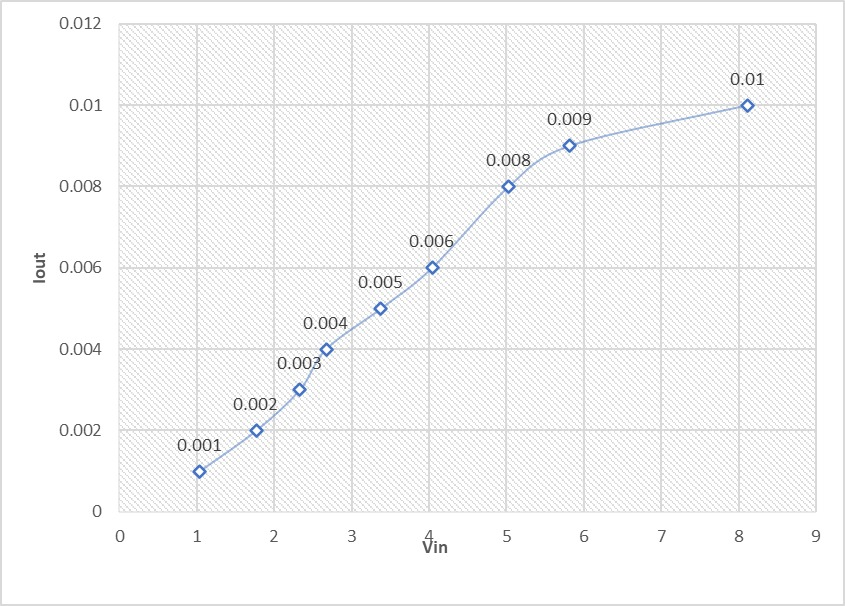
\includegraphics[scale=0.3]{src/exp02/curve1.jpeg}
    \caption{V-I characteristics Graph of 50 ohm circuit}
\end{figure}

\begin{figure}[H]
    \centering
    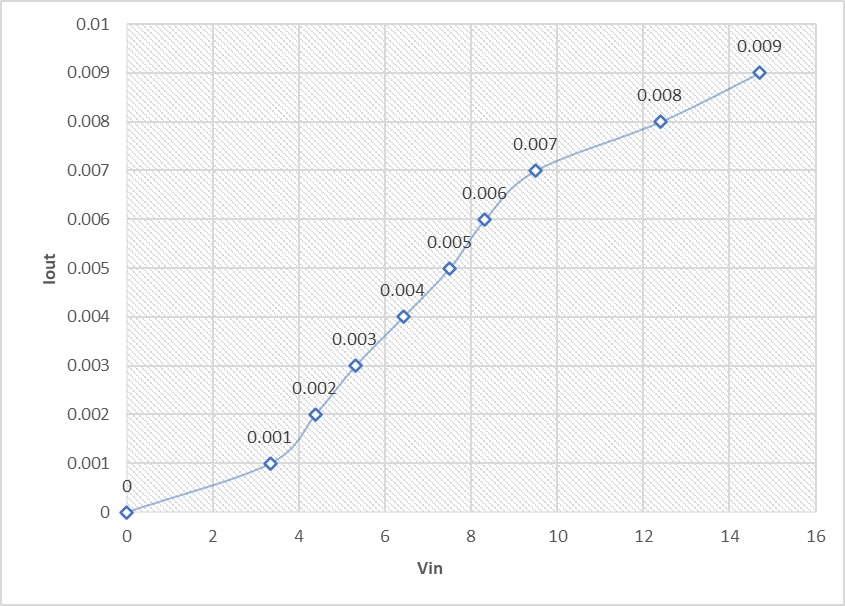
\includegraphics[scale=0.3]{src/exp02/curve2.jpeg}
    \caption{V-I characteristics Graph of 100 ohm circuit}
\end{figure}

\begin{figure}[H]
    \centering
    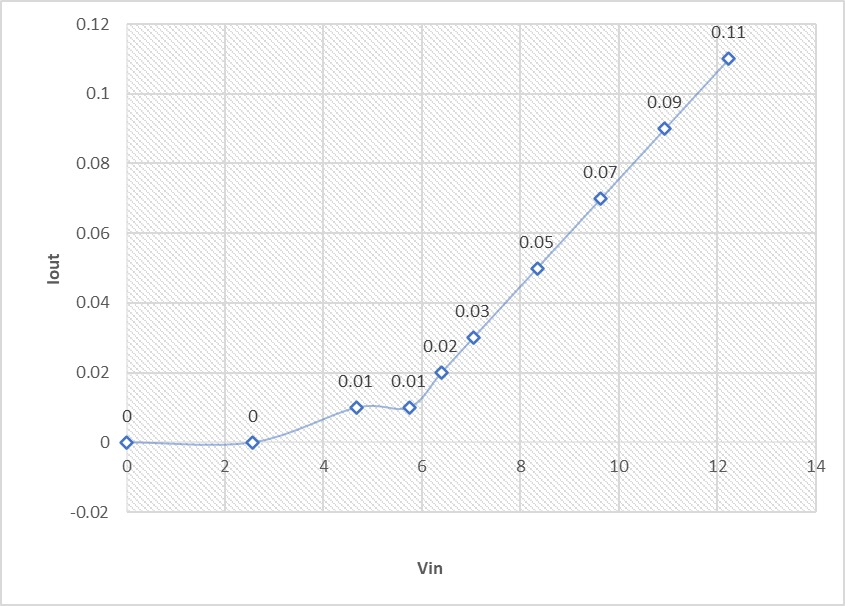
\includegraphics[scale=0.3]{src/exp02/curve3.jpeg}
    \caption{V-I characteristics Graph of 1k ohm circuit}
\end{figure}

\section{Discussion}
In this experiment, the V-I characteristics curve of a diode has been observed. Three sets of readings were taken in forward bias to plot the graphs. The voltage has been represented along the x-axis, while the current has been plotted along the y-axis. The p-type was connected to the positive terminal of the external voltage, while the n-type was connected to the negative terminal when the P-N junction diode was in forward bias condition. As the diode was in forward bias, the current has gradually risen, and as the voltage applied to the diode broke through the potential barrier, a non-linear curve should have been obtained.

\section{Conclusion}

The results indicate that the experiment was likely successful. As the voltage was increased in forward bias, the current also exhibited a corresponding increase, which is a typical diode behavior. However, the curve did not display a non-linear pattern, likely due to limited data collection. Collecting more data might have provided additional diode characteristics and insights.

